\subsubsection{World 1: Violations}
The first world presents the most important base functions of the model: it has 2 users and an
officer, all registered with different emails. The users report Violations, which have a position, a set of images
and optionally a ticket. Each local police receives a violation if its position is among the positions of the police itelf,
which form a perimeter around the city.

In each violation there is always at least an image which shows a licence plate that has been read
by the system. All the violations also have a violationType and the police system also exposes accidents along with their type.

\begin{figure}
    \noindent\makebox[\textwidth]{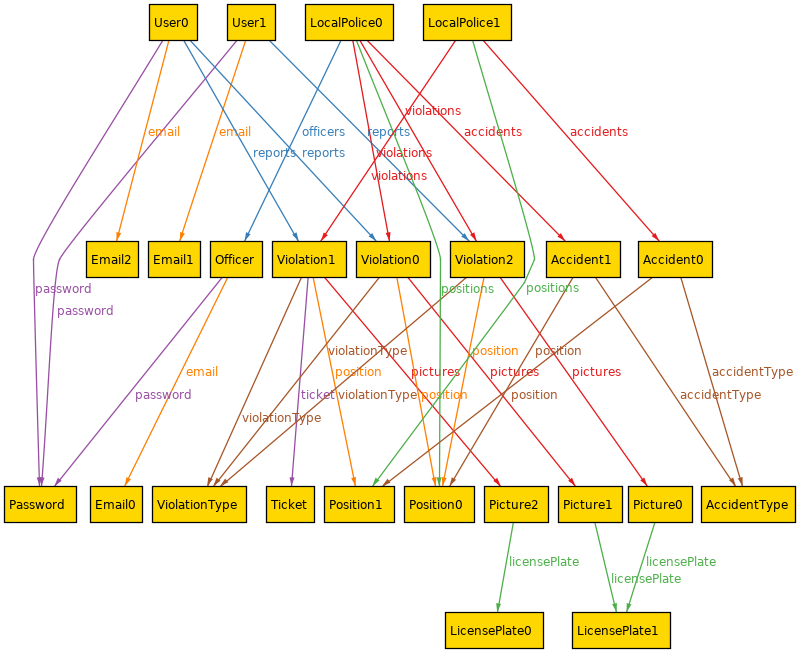
\includegraphics[width=\paperwidth]{images/worlds/world1.png}}
\end{figure}

\subsubsection{world2}
The second world shows a complete representation of the unsafe areas: each local police system gets signalled by SafeStreet
a series of unsafe area, which are connected to a position and are always in the police system handling that position.
Each unsafePosition is connected to an unsafeReason, which is itself made by a violationType an accidentType and a suggestion. This is
because the unsafeReasons are inserted by hand by operators using accident and violation categories.

The system detects an unsafe area if there are enough accidents and violations of a certain type in a position, and
suggests a possible solution.